\subsection{Transistor Kippstufen: Blinkschaltung} % (fold)
\label{sub:Transistor_Kippstufen:_Blinkschaltung}
\begin{frame}
    \frametitle{Blinkschaltung}
    \framesubtitle{Schaltung}
    \begin{figure}[H]
    \begin{center}
            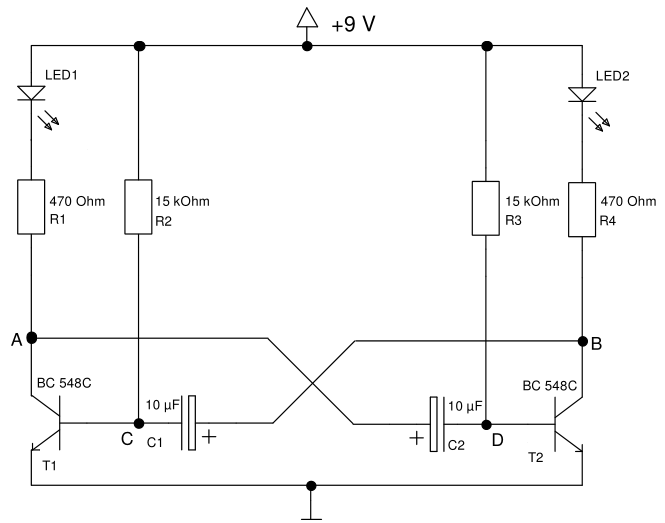
\includegraphics[scale=0.37]{./img/schaltungen/blink_0.png}
    \end{center}
    \end{figure}
\end{frame}

\begin{frame}
    \frametitle{Blinkschaltung}
    \begin{columns}[c]
    \column{.6\textwidth}    
        \begin{figure}[H]
        \begin{center}
                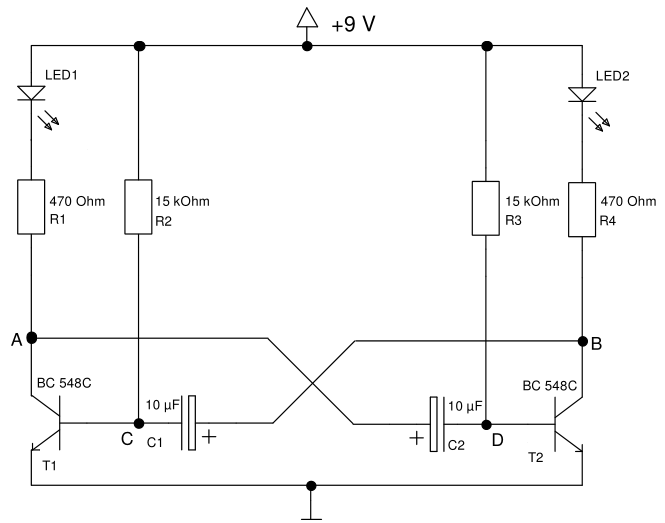
\includegraphics[scale=0.3]{./img/schaltungen/blink_0.png}
        \end{center}
        \end{figure}
    \column{.4\textwidth}    
    \begin{figure}[H]
    \begin{center}
            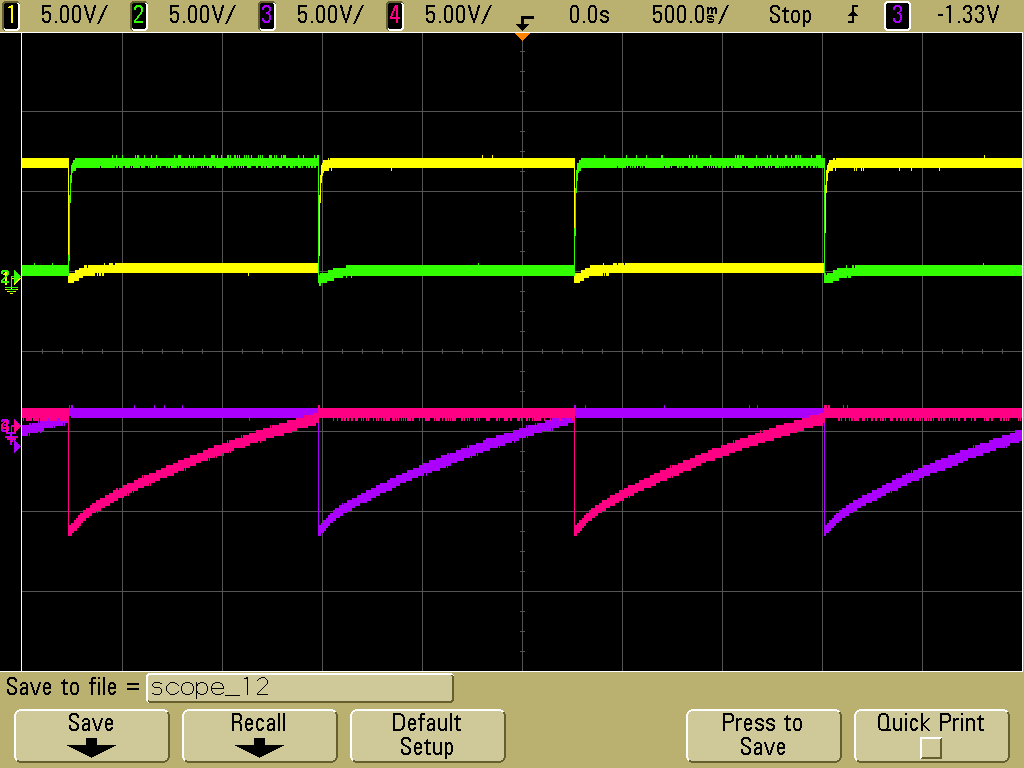
\includegraphics[scale=0.12]{./img/oszi/Aufgabe232_220kOhm_2.png}
    \end{center}
    \end{figure}
    
    \end{columns}
\end{frame}

\begin{frame}
    \frametitle{Blinkschaltung}
    \begin{columns}[c]
    \column{.6\textwidth}    
        \begin{figure}[H]
        \begin{center}
                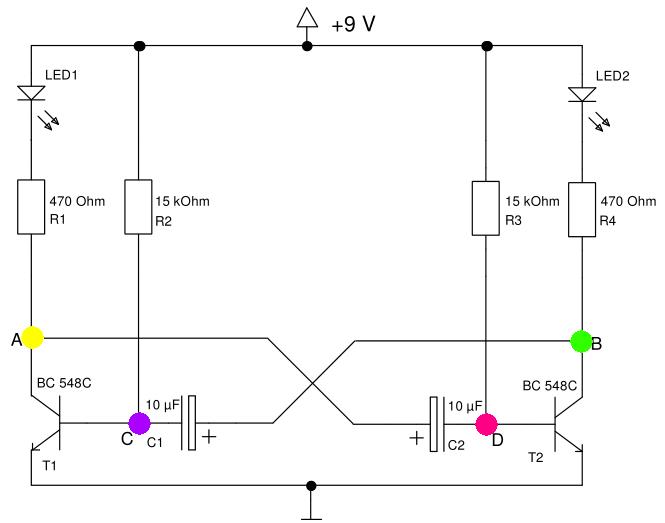
\includegraphics[scale=0.3]{./img/schaltungen/blink_1.png}
        \end{center}
        \end{figure}
    \column{.4\textwidth}    
    \begin{figure}[H]
    \begin{center}
            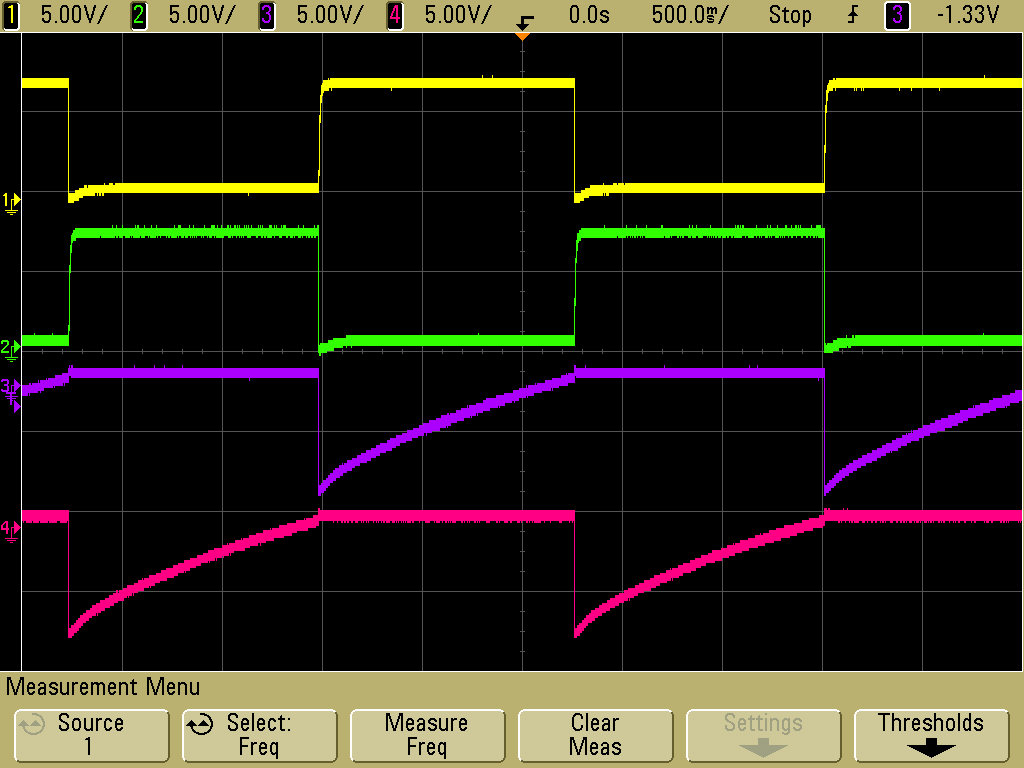
\includegraphics[scale=0.12]{./img/oszi/Aufgabe232_220kOhm_1.png}
    \end{center}
    \end{figure}
    \begin{block}{Farben}
         \begin{itemize}
             \item Gelb: A - Masse
             \item Grün: B - Masse
             \item Lila: C - Masse
             \item Rosa: D - Masse
         \end{itemize}
    \end{block}
    
    \end{columns}
\end{frame}

\begin{frame}
    \frametitle{Blinkschaltung}
    \begin{columns}[c]
    \column{.6\textwidth}    
        \begin{figure}[H]
        \begin{center}
                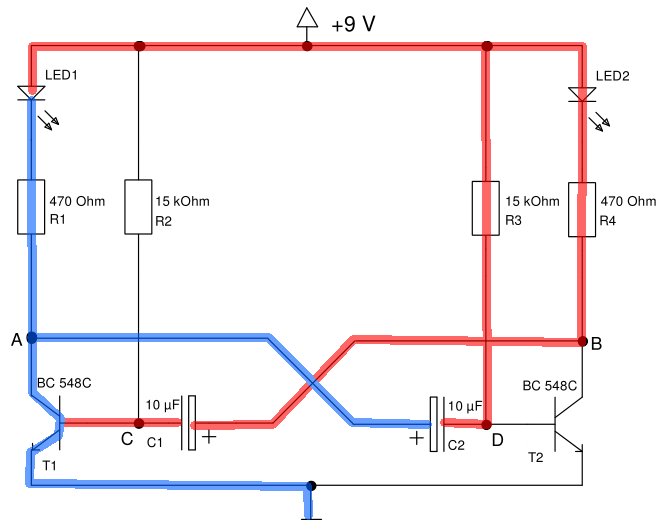
\includegraphics[scale=0.25]{./img/schaltungen/blink_2.png}
        \end{center}
        \end{figure}
    \column{.4\textwidth}    
    \begin{figure}[H]
    \begin{center}
            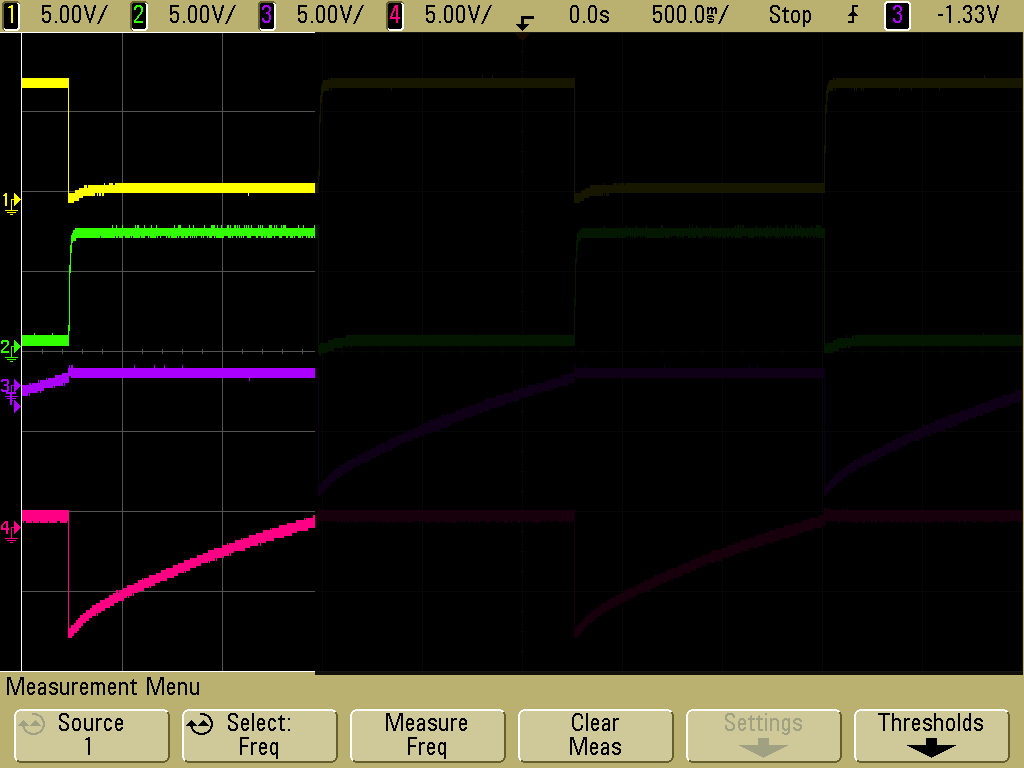
\includegraphics[scale=0.12]{./img/oszi/blink_shade_1.png}
    \end{center}
    \end{figure}
    \end{columns}
    \begin{block}{}
         \begin{itemize}
            \item Positive Spannung an $C_1$
            \item $T_1$ schaltet durch $\rightarrow$ $LED_1$ leuchtet
            \item $A$ auf Masse, $B$ auf $6.7V$
            \item Spannung zwischen $D$ und $A$ $\rightarrow$ $C_2$ wird aufgeladen
         \end{itemize}
    \end{block}
\end{frame}

\begin{frame}
    \frametitle{Blinkschaltung}
    \begin{columns}[c]
    \column{.6\textwidth}    
        \begin{figure}[H]
        \begin{center}
                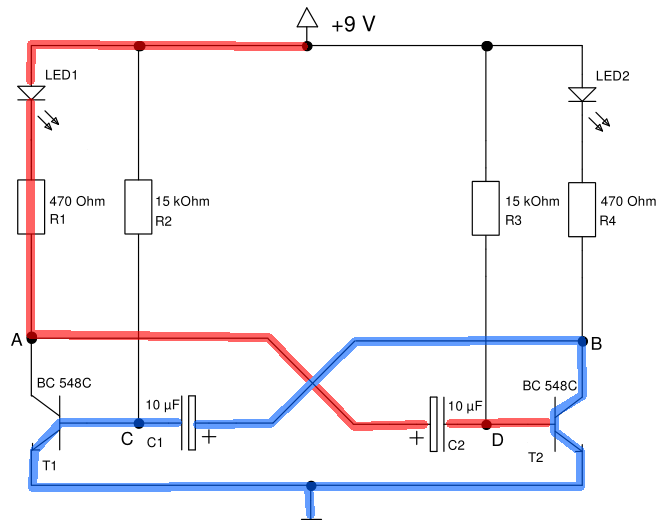
\includegraphics[scale=0.25]{./img/schaltungen/blink_3.png}
        \end{center}
        \end{figure}
    \column{.4\textwidth}    
    \begin{figure}[H]
    \begin{center}
            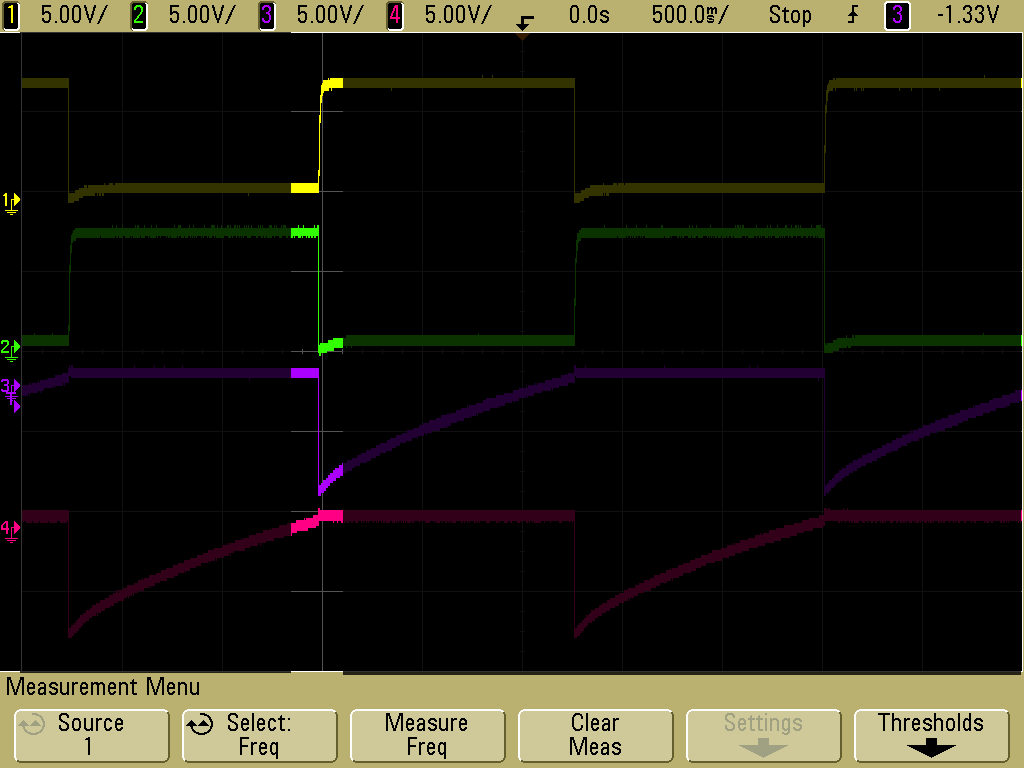
\includegraphics[scale=0.12]{./img/oszi/blink_shade_1_5.png}
    \end{center}
    \end{figure}
    \end{columns}
    \begin{block}{}
         \begin{itemize}
            \item $D$ erreicht Sperrspannung $\rightarrow$ $T_2$ schaltet durch
            \item $B$ fällt auf Masse $\rightarrow$ $C_1$ fällt ins Negative
            \item $T_1$ wird unterbrochen
         \end{itemize}
    \end{block}
\end{frame}
\begin{frame}
    \frametitle{Blinkschaltung}
    \begin{columns}[c]
    \column{.6\textwidth}    
        \begin{figure}[H]
        \begin{center}
                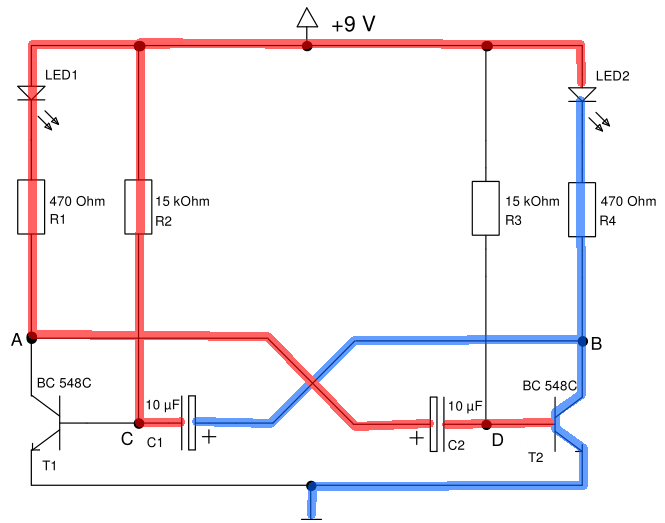
\includegraphics[scale=0.25]{./img/schaltungen/blink_4.png}
        \end{center}
        \end{figure}
    \column{.4\textwidth}    
    \begin{figure}[H]
    \begin{center}
            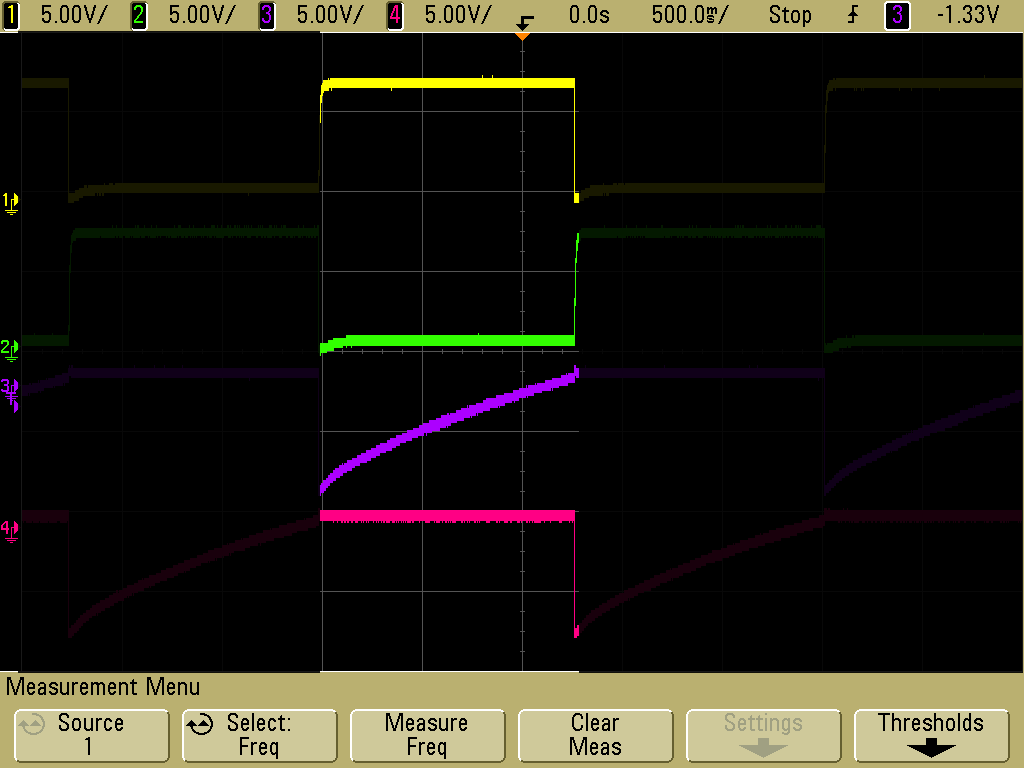
\includegraphics[scale=0.12]{./img/oszi/blink_shade_2.png}
    \end{center}
    \end{figure}
    \end{columns}
    \begin{block}{}
         \begin{itemize}
            \item Positive Spannung an $C_2$
            \item $T_2$ schaltet durch $\rightarrow$ $LED_2$ leuchtet
            \item $B$ auf Masse, $A$ auf $6.7V$
            \item Spannung zwischen $B$ und $C$ $\rightarrow$ $C_1$ wird
            aufgeladen
         \end{itemize}
    \end{block}
\end{frame}
\begin{frame}
    \frametitle{Blinkschaltung}
    \begin{columns}[c]
    \column{.6\textwidth}    
        \begin{figure}[H]
        \begin{center}
                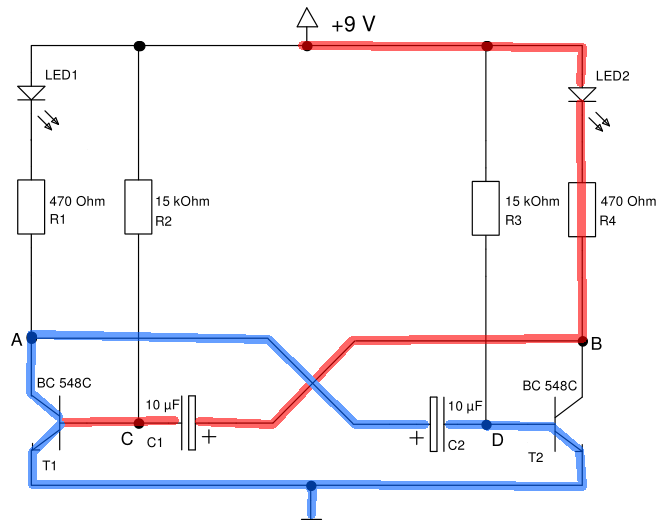
\includegraphics[scale=0.25]{./img/schaltungen/blink_5.png}
        \end{center}
        \end{figure}
    \column{.4\textwidth}    
    \begin{figure}[H]
    \begin{center}
            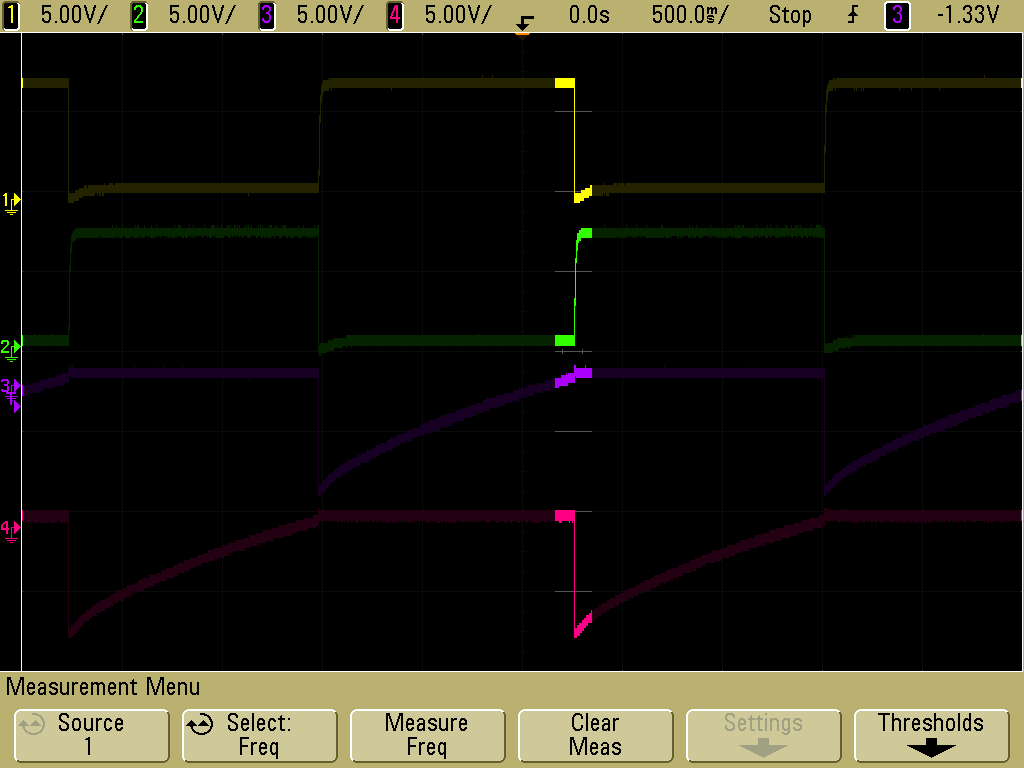
\includegraphics[scale=0.12]{./img/oszi/blink_shade_2_5.png}
    \end{center}
    \end{figure}
    \end{columns}
    \begin{block}{}
         \begin{itemize}
            \item $C$ erreicht Sperrspannung $\rightarrow$ $T_1$ schaltet durch
            \item $A$ fällt auf Masse $\rightarrow$ $C_2$ fällt ins Negative
            \item $T_2$ wird unterbrochen
         \end{itemize}
    \end{block}
\end{frame}
\begin{frame}
    \frametitle{Blinkschaltung}
    \begin{columns}[c]
    \column{.6\textwidth}    
        \begin{figure}[H]
        \begin{center}
                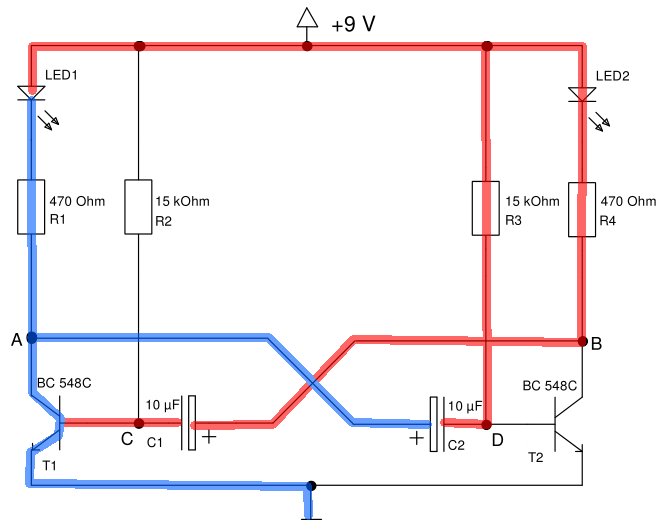
\includegraphics[scale=0.3]{./img/schaltungen/blink_2.png}
        \end{center}
        \end{figure}
    \column{.4\textwidth}    
    \begin{figure}[H]
    \begin{center}
            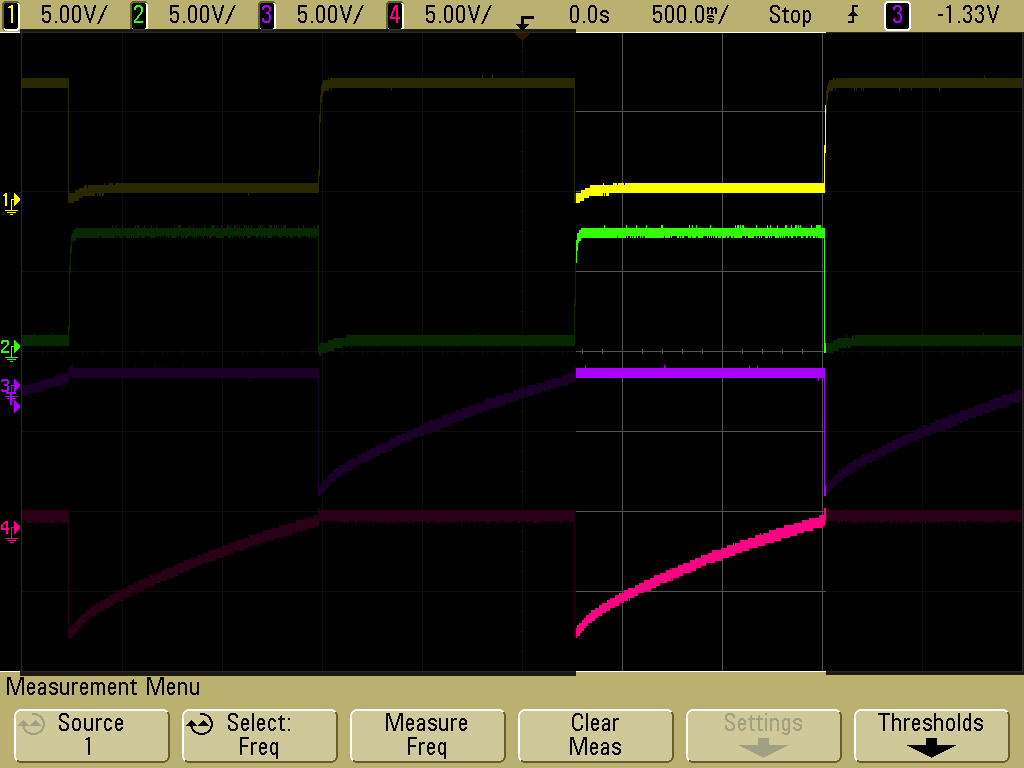
\includegraphics[scale=0.12]{./img/oszi/blink_shade_3.png}
    \end{center}
    \end{figure}
    \end{columns}
    \begin{block}{}
         \begin{itemize}
         \item Züruck beim Anfangszustand
         \end{itemize}
    \end{block}
\end{frame}
\begin{frame}
    \frametitle{Bemerkungen}
    \framesubtitle{}
    \begin{columns}[c]
    \column{0.5\textwidth} 
     \begin{block}{}
         \begin{itemize}
             \item System "schwingt" mit $\sim 395mHz$  
             \item Austauschen von Bauteilen verändert Frequenz \textbf{einer} LED
             \item Weiterhin von Interesse:
             \begin{itemize}
                 \item Einschwingvorgang ("Welche LED leuchtet zuerst?")
                 \item Abhängigkeit des Einschwingvorgangs von den Bauteilen
             \end{itemize}
         \end{itemize}
     \end{block}
     \column{0.5\textwidth}
     \begin{figure}[H]
     \begin{center}
             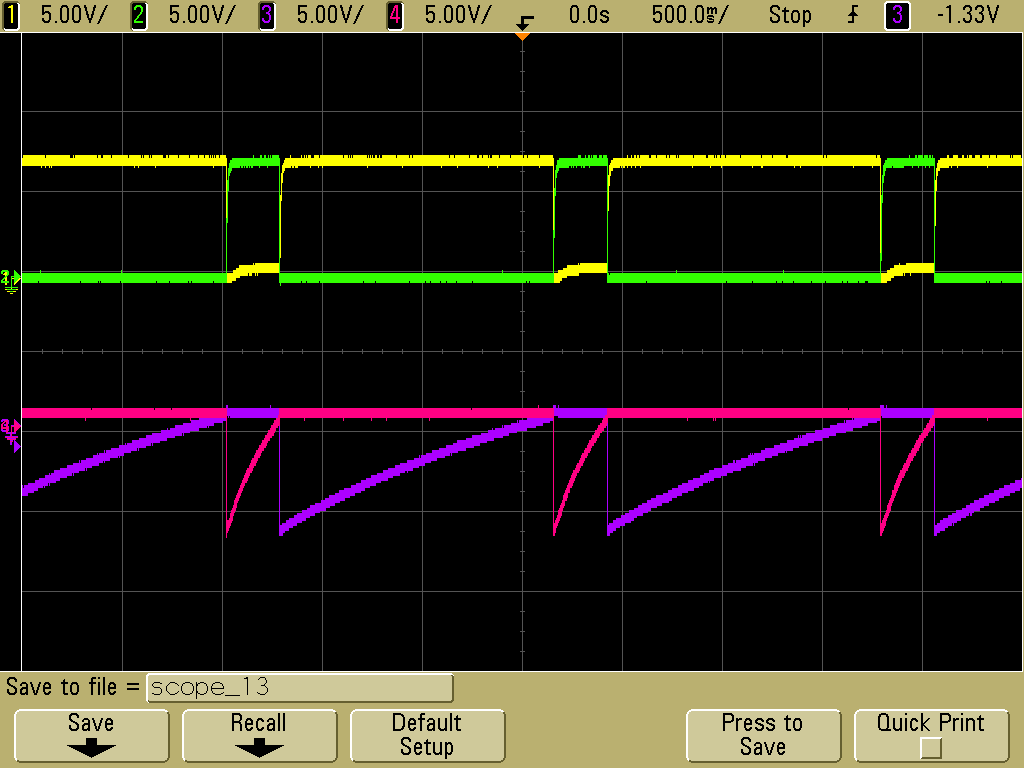
\includegraphics[scale=0.15]{./img/oszi/Aufgabe232_47kOhm.png}
     \end{center}
     \caption{Messbild mit $R_2 = 47k\Omega$}
     \end{figure}
     
    \end{columns}
\end{frame}
% section Transistor Kippstufen: Blinkschaltung (end)

